% P3, Figure F1 (manuscript Fig. 2): structure of the paired certificate, in the style of the roadmap (F0_khung.tex) and
% of the companion MSSP manuscript: white input boxes, shaded derived boxes with a bold title, a one-line statement and
% the equation, result and section; solid arrows for the computation, dashed arrows for the feedback of the policy.
% Redrawn 18/10/2026. Width 161 mm. Every box has an inner sep of 2pt (0.7 mm per side): inputs of text width 34 mm
% (x = 0 to 35.4), derived boxes of 26 mm (x = 39.4, 70.8, 102.2, 133.6 to +27.4), all derived boxes 33 mm high.
% Compile: xelatex F1_cau_truc.tex -> F1_cau_truc.pdf (copied to F1.pdf).
\documentclass{article}
\usepackage{newtxmath}
\usepackage[no-math]{fontspec}
\setmainfont{TeX Gyre Termes}
\usepackage{tikz}
\usetikzlibrary{arrows.meta}
\pagestyle{empty}
\begin{document}
\setbox0=\hbox{\fontsize{7pt}{8.4pt}\selectfont
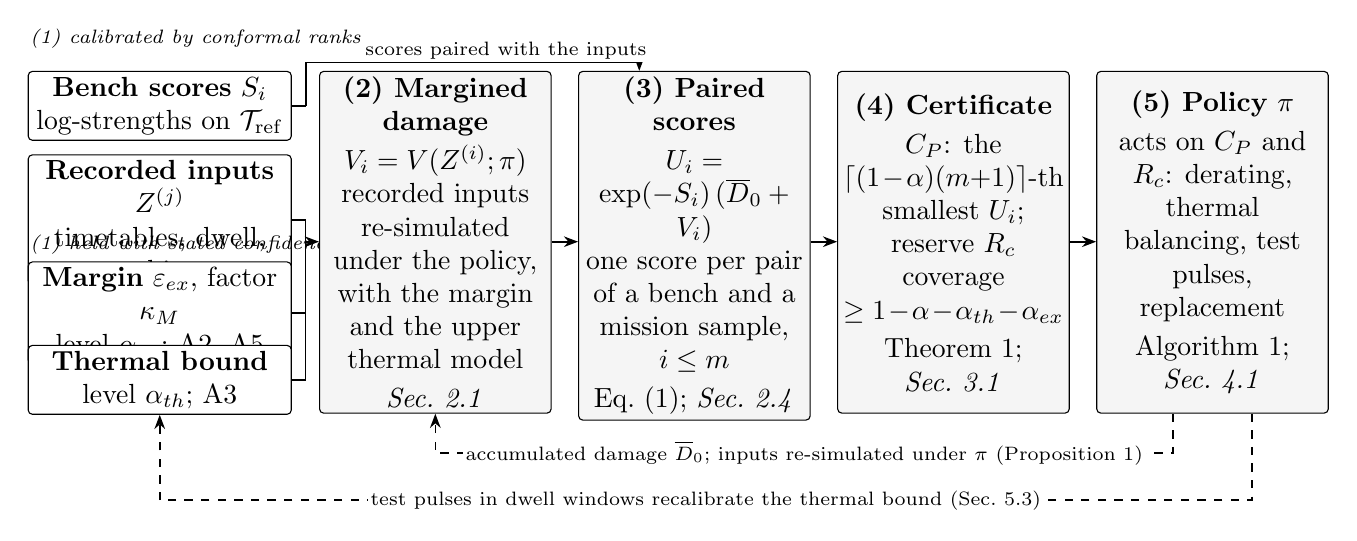
\begin{tikzpicture}[x=1mm, y=1mm,
    box/.style={draw, rounded corners=1.5pt, align=flush center, inner sep=2pt, anchor=north,
                execute at begin node={\hyphenpenalty=10000\exhyphenpenalty=10000},
                text width=#1, fill=black!4},
    box/.default=28mm,
    inp/.style={box=32mm, fill=white, minimum height=8.6mm},
    grp/.style={font=\itshape\fontsize{6.6pt}{7.6pt}\selectfont, anchor=south west, inner sep=0.5pt},
    note/.style={font=\fontsize{6.6pt}{7.6pt}\selectfont, inner sep=1pt, fill=white},
    arr/.style={-{Stealth[length=1.8mm]}, semithick},
    fb/.style={arr, dashed}]

% (1) inputs
\node[grp] at (0, 2.6) {(1) calibrated by conformal ranks};
\node[inp] (bench) at (16.7, 0)     {\textbf{Bench scores} $S_i$\\log-strengths on $\mathcal T_{\mathrm{ref}}$};
\node[inp] (miss)  at (16.7, -10.6)  {\textbf{Recorded inputs} $Z^{(j)}$\\timetables, dwell, ambient};
\node[grp] at (0, -23.6) {(1) held with stated confidence};
\node[inp] (marg)  at (16.7, -24.2) {\textbf{Margin} $\varepsilon_{ex}$, factor $\kappa_M$\\level $\alpha_{ex}$; A2, A5};
\node[inp] (therm) at (16.7, -34.8) {\textbf{Thermal bound}\\level $\alpha_{th}$; A3};

% (2)-(5) derived quantities
\node[box, minimum height=43.4mm] (V) at (51.7, 0)
  {\textbf{(2) Margined damage}\\[2pt]$V_i=V(Z^{(i)};\pi)$\\recorded inputs re-simulated under the policy, with the
   margin and the upper thermal model\\[2pt]\textit{Sec.~2.1}};
\node[box, minimum height=43.4mm] (U) at (84.6, 0)
  {\textbf{(3) Paired scores}\\[2pt]$U_i=\exp(-S_i)\,(\overline D_0+V_i)$\\one score per pair of a bench and a mission
   sample, $i\le m$\\[2pt]Eq.~(1); \textit{Sec.~2.4}};
\node[box, minimum height=43.4mm] (C) at (117.5, 0)
  {\textbf{(4) Certificate}\\[2pt]$C_P$: the $\lceil(1-\alpha)(m{+}1)\rceil$-th smallest $U_i$; reserve $R_c$\\coverage
   $\ge1-\alpha-\alpha_{th}-\alpha_{ex}$\\[2pt]Theorem~1; \textit{Sec.~3.1}};
\node[box, minimum height=43.4mm] (P) at (150.4, 0)
  {\textbf{(5) Policy} $\pi$\\[2pt]acts on $C_P$ and $R_c$: derating, thermal balancing, test pulses, replacement\\[2pt]
   Algorithm~1; \textit{Sec.~4.1}};

% computation
\coordinate (j) at (35.2, -21.7);
\draw[semithick] (miss.east) -| (j);
\draw[semithick] (marg.east) -| (j);
\draw[semithick] (therm.east) -| (j);
\draw[arr] (j) -- (j -| V.west);
\draw[semithick] (bench.east) -- ++(1.8,0) coordinate (b1);
\draw[arr] (b1) |- ++(0,5.5) -| node[note, pos=0.3, above]{scores paired with the inputs} ([xshift=-7mm]U.north);
\draw[arr] (V.east |- 0,-21.7) -- (U.west |- 0,-21.7);
\draw[arr] (U.east |- 0,-21.7) -- (C.west |- 0,-21.7);
\draw[arr] (C.east |- 0,-21.7) -- (P.west |- 0,-21.7);

% feedback of the policy
\draw[fb] ([xshift=-5mm]P.south) -- ++(0,-5) -| node[note, pos=0.25]{accumulated damage $\overline D_0$; inputs re-simulated under $\pi$ (Proposition~1)} (V.south);
\draw[fb] ([xshift=5mm]P.south) -- ++(0,-11) -| node[note, pos=0.25]{test pulses in dwell windows recalibrate the thermal bound (Sec.~5.3)} (therm.south);
\end{tikzpicture}}
\pdfpagewidth=\dimexpr\wd0+4pt\relax
\pdfpageheight=\dimexpr\ht0+\dp0+4pt\relax
\shipout\vbox{\vskip-1in\vskip2pt\hbox{\hskip-1in\hskip2pt\box0}}
\end{document}
